\section{A complete curved polynomial example}\label{sec:example}

Consider the upward-oriented patch
\[
 \sigma(u,v)=(u,v,uv),\qquad 0\le u,v\le1,
\]
and the vector field
\[
 \mathbf F(x,y,z)=(0,xz,x^2y).
\]
These are rational polynomials on the relevant unit boxes. Exact evaluation,
all derivative programs, and the certificates of
\cref{sec:polynomial-jets} are available by finite arithmetic.
The normal area vector is
\[
 \sigma_u=(1,0,v),\qquad \sigma_v=(0,1,u),\qquad
 \sigma_u\times\sigma_v=(-v,-u,1).
\]
Its third coordinate is one, so there is no degeneracy or orientation
ambiguity in this particular surface presentation.

\subsection{Pullback and curl calculation}

The pulled-back one-form is
\[
 \sigma^*(\mathbf F\cdot\dd\mathbf r)=P\,\dd u+Q\,\dd v,
 \qquad
 P=u^2v^2,\qquad Q=u^2v(1+u).
\]
Indeed $\mathbf F(\sigma)=(0,u^2v,u^2v)$, and taking its dot products
with the two tangent vectors gives these expressions.
Differentiating the finite polynomials gives
\[
 \partial_uQ-\partial_vP=(2u+3u^2)v-2u^2v=uv(u+2).
\]
Independently,
\[
 \curl\mathbf F=(x^2-x,-2xy,z),
\]
and
\[
 (\curl\mathbf F)(\sigma)\cdot(-v,-u,1)
 =-(u^2-u)v+2u^2v+uv=uv(u+2).
\]
This checks both curvature and a nonconstant curl integrand; it is not
an example in which the surface dependence disappears trivially.

\subsection{Boundary values and exact integral}

The four counterclockwise edges give
\[
 \begin{array}{c|c|c}
 \text{edge}&\text{oriented integrand}&\text{integral}\\ \hline
 v=0,\ u:0\to1&0&0\\
 u=1,\ v:0\to1&2v&1\\
 v=1,\ u:1\to0&-u^2\text{ on }[0,1]&-1/3\\
 u=0,\ v:1\to0&0&0
 \end{array}
\]
Thus the boundary integral is $2/3$. The volume side is also $2/3$.
This statement can be checked without assuming ordinary integration
formulas: the following finite-sum identities explicitly construct the
two names and their common rational value.

\subsection{Every Riemann sum in closed form}

Use exact evaluation and $N$ equal intervals in each parameter direction.
The finite identities
\[
 \sum_{a<N}a=\frac{N(N-1)}2,\qquad
 \sum_{a<N}a^2=\frac{N(N-1)(2N-1)}6
\]
are proved by quantifier-free induction after clearing denominators.
Substitution in the definitions of $V$ and $B$ yields
\begin{align}
 V_N&=\frac{(N-1)^2(8N-1)}{12N^3},\label{eq:example-V}\\
 B_N&=\frac{(N-1)(4N+1)}{6N^2},\label{eq:example-B}\\
 B_N-V_N&=\frac{(N-1)(11N-1)}{12N^3}.\label{eq:example-defect}
\end{align}
In particular, the two sums are generally different at a finite mesh.
Stokes is equality of their represented integrals, not an assertion that
the derivative Riemann sum equals the boundary Riemann sum at every mesh.
The difference sum $T_N$, in contrast, equals $B_N$ exactly.

The exact errors relative to the common value are
\[
 \frac23-V_N=\frac{17N^2-10N+1}{12N^3},\qquad
 \frac23-B_N=\frac{3N+1}{6N^2}.
\]
For $N\ge1$ these are nonnegative and at most $17/(12N)$ and $2/(3N)$,
respectively. Taking $N\ge2^{r+1}$ makes each error smaller than $2^{-r}$.
This directly verifies the named integral value $2/3$.

\begin{table}[ht]
\centering
\caption{Exactly computed left-grid sums for the curved example.
The decimal columns are only for readability; the validation uses fractions.}
\begin{tabular}{r r r r}
\toprule
$N$&$V_N$&$B_N=T_N$&$B_N-V_N$\\
\midrule
2&0.156250000&0.375000000&0.218750000\\
4&0.363281250&0.531250000&0.167968750\\
8&0.502441406&0.601562500&0.099121094\\
16&0.581359863&0.634765625&0.053405762\\
32&0.623207092&0.650878906&0.027671814\\
\bottomrule
\end{tabular}
\end{table}

\begin{figure}[htbp]
\centering
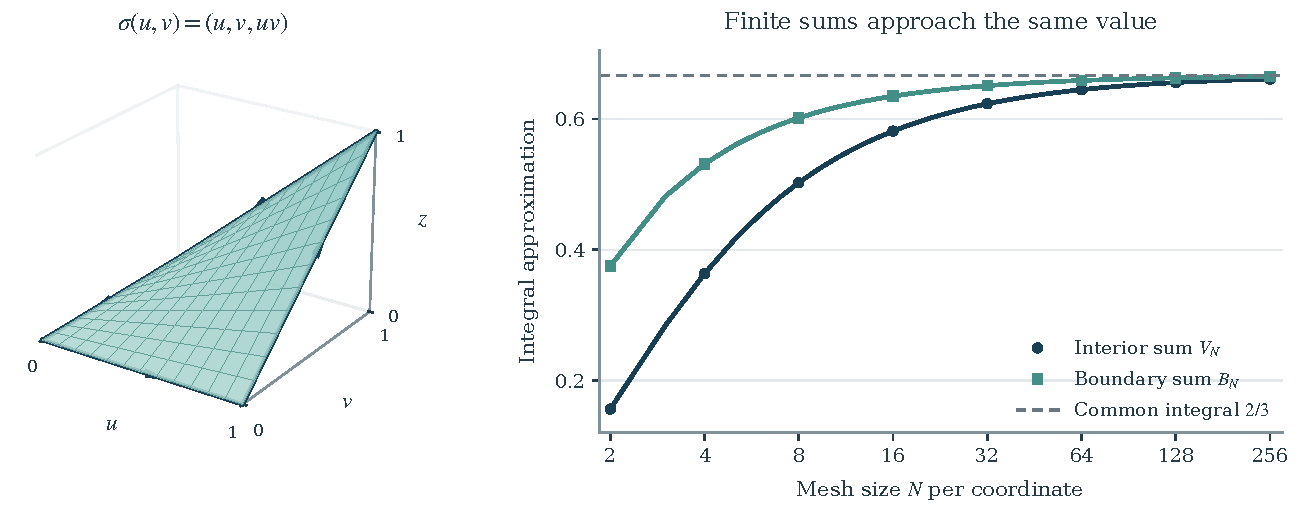
\includegraphics[width=\textwidth]{figures/example_convergence.pdf}
\caption{The curved polynomial patch and its two independently defined
Riemann sums. The common target $2/3$ and the plotted values follow from
the exact rational formulas \eqref{eq:example-V} and \eqref{eq:example-B}.}
\label{fig:example}
\end{figure}

\subsection{Explicit certificates for this example}

The cube flux coefficients and their relevant derivatives are
\[
 f_1=u^2v+u^3v,\quad f_2=-u^2v^2,\quad
 g_1=(2u+3u^2)v,\quad g_2=-2u^2v.
\]
On $Q^2$, their sup-norm Lipschitz bounds are respectively $7,4,13,6$.
For example, on $[0,1]$ the factorization of $a^j-b^j$ gives
$|a^j-b^j|\le j|a-b|$; applying it to each factor in a monomial proves
these constants directly. A common continuity modulus is therefore
\[
 \mu_F(t)=\mu_G(t)=t+4.
\]
Their exact coordinate remainders are
\[
 R_1=vh^2(1+3u+h),\qquad R_2=-u^2h^2.
\]
For an admissible forward $u$-increment, $u+h\le1$, so
$1+3u+h\le4$. Hence $|R_1|\le4h^2$ and $|R_2|\le h^2$.
A common modulus is $\tau(t)=t+2$.

For $k=2$, $\ell(k)=1$, and the general schedule becomes
\[
 t_r=r+5,\qquad n_r=r+9,\qquad N_r=2^{r+9},\qquad p_r=2r+16.
\]
The general finite error budget simplifies exactly to
\[
 \frac{2\,2^{-t_r}+2(2N_r+1)2^{-p_r}}{2^{-r}}
       =\frac3{32}+2^{-r-15}<\frac18.
\]
The exact polynomial values make the evaluation part unnecessary in this
example, so this general bound is deliberately conservative. Its purpose
is to demonstrate the uniform recipe that also works with rounded
coefficient data.

\FloatBarrier
\section{Executable checks and their limits}\label{sec:checks}

The archive contains a Python reference implementation using the standard
library's \path{fractions.Fraction}. It evaluates the finite expressions
$V,B,T$, polynomial coefficients, and cubical boundaries. The independent
validation run recorded the following successful checks:

\begin{center}
\begin{tabular}{p{0.68\textwidth}r}
\toprule
Check & Cases\\
\midrule
Exact telescoping on arbitrary rational sampled tables in dimensions
$1$ through $4$ &36\\
Cancellation of every codimension-two coefficient in $\partial^2$
for dimensions $2$ through $6$ &5\\
Direct enumeration of the curved example at $N=1,2,4,8,16,32$,
compared with the closed formulas &6\\
Rounded dyadic evaluations satisfying the local remainder contract
and the global error bound &48\\
Large precision schedules checked by the independently verified
closed formulas &19\\
\bottomrule
\end{tabular}
\end{center}

The polynomial recurrence identities, the pullback/curl identity, and
the two displayed Taylor remainders were checked by equality of complete
finite coefficient dictionaries. They were not inferred from agreement
at sampled points. The large schedule cases use the closed formulas;
their enormous grids were not enumerated.

These checks catch orientation, scaling, endpoint, and precision-accounting
errors. They are not proofs of a universally quantified theorem, and they
do not replace the human proof or an internal iPRA derivation. Python
callables are an execution interface; the proof-theoretic claim applies
to their fixed primitive recursive mathematical instances.

The JSON receipt includes the source hashes and the exact fractions.
The CSV tables contain the direct-grid and schedule results.
The plotting script is a separate optional dependency on Matplotlib;
the validation itself has no external Python dependencies.
